\section{\large\textbf{Methodology}}
\subsection{Sound stimuli}

The stimuli were auralized, as this methodology allows for precise control of the source directivity. They consist of pink noise filtered in one-third octave bands, with an 8-second fade-in to eliminate impulsive effects. In the present study, three types of constant directivity sources were used, with $Q$ values of 1, 2, and 4. The directivity values were selected considering the high cost and impracticality of achieving greater directivity within this frequency range in a home surround sound system. For the room acoustics, the data from the study conducted by \textcite{jackson} were employed, generating a space with reverberation times and average volume corresponding to a living room.

The dimensions of the simulated room are 4.3 m × 4.3 m × 2.4 m, yielding a total volume of $44.4~\text{m}^3$. All surfaces were assigned an average absorption coefficient calculated from the study data. In addition, linear interpolations were performed between octave bands to assign absorption coefficients in one-third octave bands.

Since ray tracing is used for the auralization, this technique is valid for frequencies above the Schroeder frequency. For the simulated room, this frequency is 220 Hz. Therefore, the range of the stimuli spans from the one-third octave band of 250 Hz to 1250 Hz. For lower frequencies, a simulation based on the wave equation would be required.

The source arrangement follows an equilateral triangle with the listener at its center. The sources are positioned more than half a wavelength of the lowest frequency under study away from the walls (70 cm) to avoid unwanted variations in the source directivity. The height of the sources matches that of the listener, with both placed at 1.2 m.
The impulse responses were calculated considering reflections up to the 12th order. Subsequently, the stimuli were processed for binauralization, resulting in 8 stimulus pairs per source, yielding a total of 24 pairs. Figure \ref{fig:BRIRS} presents the binaural impulse responses for the left source as an example.

Due to the symmetry employed, the binaural response for the right source is identical but with inverted channels. Each impulse response includes a reverberation tail designed according to the initial slope of early reflections, ensuring consistency with the space's acoustic characteristics.
\begin{figure}[H]
    \centering
    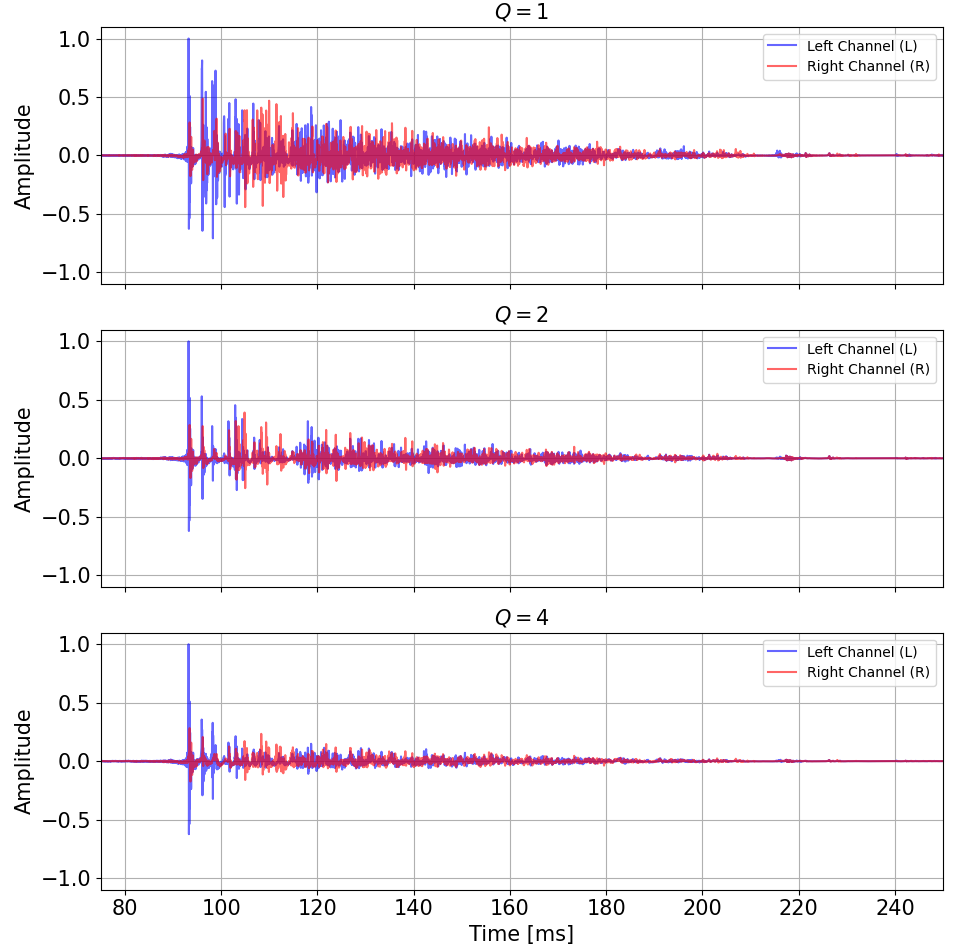
\includegraphics[width=0.65\textwidth]{Figures/BRIRS.png}
    \caption{Binaural impulse responses obtained.}
    \label{fig:BRIRS}
\end{figure}

\subsection{Objetive parameter}

In a room, reverberant energy significantly impairs the ability to localize sound sources, as it alters the ILD and ITD parameters due to reflections. This study aims to modify the source directivity to reduce the energy radiated towards the room, thereby mitigating this effect.

By varying the source directivity factor, the ratio between direct and reverberant energy is modified. The D/R ratio is the objective parameter of this research. Table \ref{tab:d/r} presents the D/R values obtained for each source from the impulse responses.

\begin{table}[h]
    \centering
    \caption{Values of D/R obtained for each directivity factor.}
    \begin{tabular}{c c}\hline
        Q & $D/R$ [dB] \\ \hline
        1 & -8.6       \\
        2 & -2.8       \\
        4 & 0.2        \\ \hline
    \end{tabular}
    \label{tab:d/r}
\end{table}

As can be observed, the more directive the source, the greater the direct energy relative to the reverberant energy perceived. This helps minimize the impact on binaural parameters, resulting in more accurate source localization.

\subsection{Test method}

The test to be performed involves presenting an audio stimulus from the left or right source. The source is selected randomly for each audio. The presented stimuli correspond to the third-octave bands under study and each source directivity. The participant will be asked to indicate which source the sound is coming from.

As mentioned earlier, the stimuli consist of pink noise filtered digitally into one-third octave bands using 72 dB/oct. Butterworth filters, with an 8-second fade-in and a total duration of 12 seconds. Figure \ref{fig:estimulo} shows the result of the binauralization of a 400 Hz one-third octave stimulus with the BRIR, as an example.

The stimuli are presented in three groups, labeled A, B, and C, each corresponding to a different type of source, with directivity factors of 1, 2, and 4, respectively. Each group contains eight stimuli, one for each one-third octave band. Thus, the participant will listen to 24 stimuli, each lasting 12 seconds, leading to an approximate test duration of 5 minutes. The source reproducing the stimuli was randomly selected using Python code. The sequence and final configuration were stored for further analysis.

\begin{figure}[H]
    \centering
    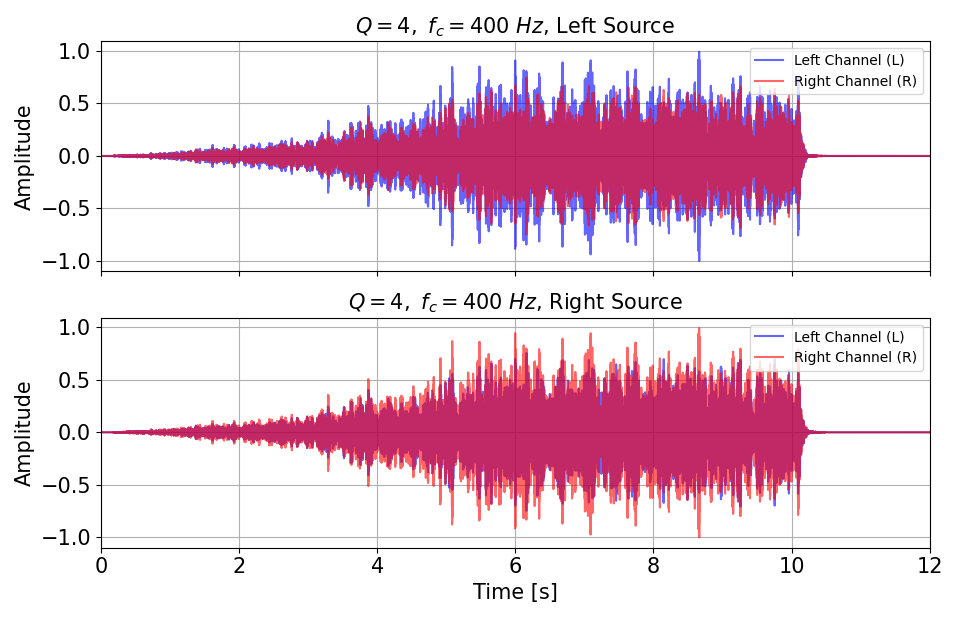
\includegraphics[width=0.65\textwidth]{Figures/Imagen1.png}
    \caption{Stimuli of third-octave pink noise centered at 400 Hz convolved with BRIR.}
    \label{fig:estimulo}
\end{figure}

Participants must not have hearing impairments and are required to use headphones to complete the test, as it will be conducted online. Additionally, a trial stimulus will be provided at the beginning to adjust the playback level, ensuring it remains constant throughout the test. The trial stimulus consists of pink noise filtered in the 1250 Hz third-octave band, as this frequency is used for the stimulus to be presented, given that it lies within a region of high auditory sensitivity. The user is recommended to start with the minimum level and increase it until reaching a level that does not cause discomfort.

For the post-analysis of the results, participants will also complete a questionnaire to segment the data and conduct differentiated analyses if necessary. The questionnaire will include the following questions:

\begin{enumerate}[label=\alph*)]
    \item Do you usually listen to surround sound systems? How often?
    \item Do you usually listen to music with headphones? How often?
    \item What equipment are you using to conduct the test?
    \item What type of headphones are you using?
    \item Do you work or study something related to sound?
    \item Are you taking the test in a noisy environment?
\end{enumerate}
As the stimuli are presented, participants complete an online survey, indicating where they perceived the sound was coming from between two options, left or right.
